\documentclass[a4paper, 11pt]{article}
\usepackage[utf8]{inputenc}


\usepackage[table]{xcolor}
\usepackage{times}
\usepackage[unicode]{hyperref}
\usepackage[left=2cm,top=3cm,text={17cm, 24cm}]{geometry}

\usepackage{graphicx}
\usepackage[table,xcdraw]{}
\usepackage{changepage}
\usepackage{rotating}
\usepackage{lmodern}
\usepackage{pdflscape}
\usepackage{changepage}
\usepackage{stackrel}
\usepackage{pdflscape}
\usepackage[czech]{babel}

%%%%%%%%%%%%%%%%%%%%%%%%%% BEGIN TITLE PAGE %%%%%%%%%%%%%%%%%%%%%%%%%%%%%% 
\begin{document}
\begin{titlepage}
\begin{center}

\includegraphics[width=0.77\linewidth]{src/FIT_logo.pdf} \\

{\Huge Dokumentace k projektu do IFJ / IAL \\ \huge Implementace překladače imperativního jazyka IFJ19}
\vspace{\stretch{0.518}}

{\huge 11. prosince 2019\\
\vspace{\stretch{0.050}}

\Huge Tým 120, varianta II}


\vspace{\stretch{0.618}}
\Large
\centering
\begin{tabular}{ll}
Autoři: & \\
Březina Jindřich - 25\% & \href{mailto:xbrezi21@stud.fit.vutbr.cz}{\texttt{xbrezi21@stud.fit.vutbr.cz}} \\
Gumančík Pavol - 25\%  & \href{mailto:xguman01@stud.fit.vutbr.cz}{\texttt{xguman01@stud.fit.vutbr.cz}} \\
Kotáb Dominik - 25\%   & \href{mailto:xkotab01@stud.fit.vutbr.cz}{\texttt{xkotab01@stud.fit.vutbr.cz}} \\
Moravčík Tomáš - vedoucí - 25\%  & \href{mailto:xmorav41@stud.fit.vutbr.cz}{\texttt{xmorav41@stud.fit.vutbr.cz}}
\end{tabular}

\end{center}
\end{titlepage}

%%%%%%%%%%%%%%%%%%%%%%%%%% ENDE TITLE PAGE %%%%%%%%%%%%%%%%%%%%%%%%%%%%%% 
\tableofcontents
\newpage

%%%%%%%%%%%%%%%%%%%%%%%%%% UVOD %%%%%%%%%%%%%%%%%%%%%%%%%%%%%%%%%%%%%%%%% 
\section{Úvod}
Tato dokumentace popisuje návrh a implementaci překladače imperativního jazyka IFJ19, který je zjednodušenou podmnožinou jazyka Python 3. Naše varianta zadání II, měla za úkol implementovat tabulku symbolů, která se nachází v souboru \verb|symtable.c| a \verb|symtable.h| pomocí tabulky s rozptýlenými položkami.

%%%%%%%%%%%%%%%%%%%%%%%%%% IMPLEMENTACE %%%%%%%%%%%%%%%%%%%%%%%%%%%%%%%%% 
\section{Implementace}
\subsection{Části překladače}
\begin{itemize}
\item Lexikální analyzátor
\item Syntaktický analyzátor
\item Sémantický analyzátor
\item Generátor kódu
\end{itemize}

\subsection{Lexikální analyzátor}
Lexikální analyzátor, ve zdrojových souborech \verb|scanner.c|, je první část překladače, která pracuje se zdrojovým textem. Čte a rozděluje jednotlivé lexémy na tokeny, se kterými dál pracuje syntaktický analyzátor. Lexikální analyzátor jsme implementovali dle našeho konečného automatu, zpracovává znak po znaku ze vstupu a na základě stavu, ve kterém skončil určí typ a případně hodnotu tokenu. Pokud při zpracovávání dostane lexikální analyzátor znak, se kterým konečný automat nepočítá, mohou nastat dvě věci:
\begin{itemize}
\item ukončí se tvorba aktuálního tokenu podle platného konečného stavu automatu a načtený znak se odloží zpátky na vstup
\item tvorba tokenu neskončila v platném konečném stavu automatu, lexikální analyzátor toto rozezná jako lexikální chybu a pošle příkaz k ukončení překladu (error code 1)
\end{itemize}

\subsection{Syntaktický analyzátor}
Syntaktický analyzátor, ve zdrojových souborech \verb|parser.c|, je hlavní částí překladače a volá všechny ostatní části překladače imperativního jazyka. Syntaktická analýza je řešena metodou rekurzivního sestupu za pomoci LL tabulky. Pro zpracování výrazů jsme využili syntaktickou analýzu shora dolu. Výrazy jsou zpravované pomocí precedenční syntaktické analýzy.

\subsection{Sémantický analyzátor}
Sémantický analyzátor je podčástí syntaktického analyzátoru. Sémantický analyzátor vyhodnocuje, zda funkce či proměnná nebyla již dříve na stejné úrovni definovaná. Funkce mohou být definované jen v globální tabulce, kdežto proměnné se mohou vyskytovat jak v globální, tak i v lokální tabulce.

\subsection{Generátor kódu}
Instrukce pro generátor kódu, ve zdrojových souborech \verb|generator.c|, jsou vytvářeny průběžně za běhu překladače a jsou ukládány do listu, ze kterého potom generátor čerpá. Generátor je volán pomocí jednotlivých tříadresných instrukcí, který generuje cílový jazyk IFJcode19.


%%%%%%%%%%%%%%%%%%%%%%%%%% ALGORITMY %%%%%%%%%%%%%%%%%%%%%%%%%%%%%%%%%%% 
\section{Algoritmy}

\subsection{Tabulka symbolů}
Tabulka symbolů, ve zdrojových souborech \verb|symtable.c|, slouží k uchování názvů definovaných funkcí a proměnných. Pro nalezení definované položky v řídkém seznamu slouží tzv. hash, který nám řekne, kde se v tabulce tato položka podle názvu nachází. U proměnné můžeme najít její přiřazenou hodnotu a u funkce její jednotlivé argumenty nebo definované proměnné uvnitř této funkce.

\subsection{Zásobníky}
V naší implementaci používáme dva různé zásobníky, ve zdrojových souborech \verb|stack.c| a \verb|tokenStack.c|. \verb|stack.c| v sobě uchovává hodnoty indentů. Zásobník naplňuje lexikální analyzátor a správnost indentů následně kontroluje syntaktický analyzátor. \verb|tokenStack.c| slouží syntaktické analýze výrazů. Analyzátor výrazů ukládá tokeny na zásobník tokenů a porovnává je se vstupními tokeny.

\subsection{Precedenční syntaktický algoritmus}
Precedenční syntaktický algoritmus je sice nejméně efektivní, ale využili jsme ho kvůli jednoduchosti implementace, práce s ním a taky kvůli dřívějšímu obeznámení na přednáškách IFJ.

%%%%%%%%%%%%%%%%%%%%%%%%%% VERZOVACI SYSTEM %%%%%%%%%%%%%%%%%%%%%%%%%%%%%% 

\section{Verzovací systém}
Pro jednoduchou kontrolu verzí a možnost návratu při případné chybě jsme používali technologii Git s repositářem umístěným na stránce Github. Díky tomuto projektu jsme se konečně všichni naučili správně využívat textové editory propojenými se vzdáleným repositářem, jelikož doposud jsme nebyly donuceni se s tímto seznámit.

%%%%%%%%%%%%%%%%%%%%%%%%%% KOMUNIKACE %%%%%%%%%%%%%%%%%%%%%%%%%%%%%% 

\section{Komunikace}
S komunikací jsme neměli žádné problémy, samotné programování jsme absolvovali v pokoji našeho velitele, kde jsme vzorně programovali a pokud jsme měli nějaké problémy, mohli jsme se jednoduše svěřit jednomu ze svých kolegů. Vysvětlení našeho problému většinou stačilo nám samotným k tomu, aby jsme problém identifikovali a nakonec vyřešili. Když jsme neměli po boku jeden druhého, spojoval nás komunikační kanál discord, kde jsme využívali jak písemný, tak voice chat.

%%%%%%%%%%%%%%%%%%%%%%%%%% ZAVER %%%%%%%%%%%%%%%%%%%%%%%%%%%%%% 

\section{Závěr}
Fungování překladače imperativního jazyka by mělo vyhovovat požadovanému zadání bez rozšíření. Dříve jsme zvažovali, že základní program rozšíříme o nějaké to ze snadnějších rozšíření, bohužel nakonec jsme byly rádi, že jsme zvládli samotný základní program.


%%%%%%%%%%%%%%%%%%%%%%%%%% FSM %%%%%%%%%%%%%%%%%%%%%%%%%%%%%%%%%%%%%% 

\newpage
\section{Diagram konečného automatu}
\begin{figure}[ht]
  \centering
    \scalebox{0.45}{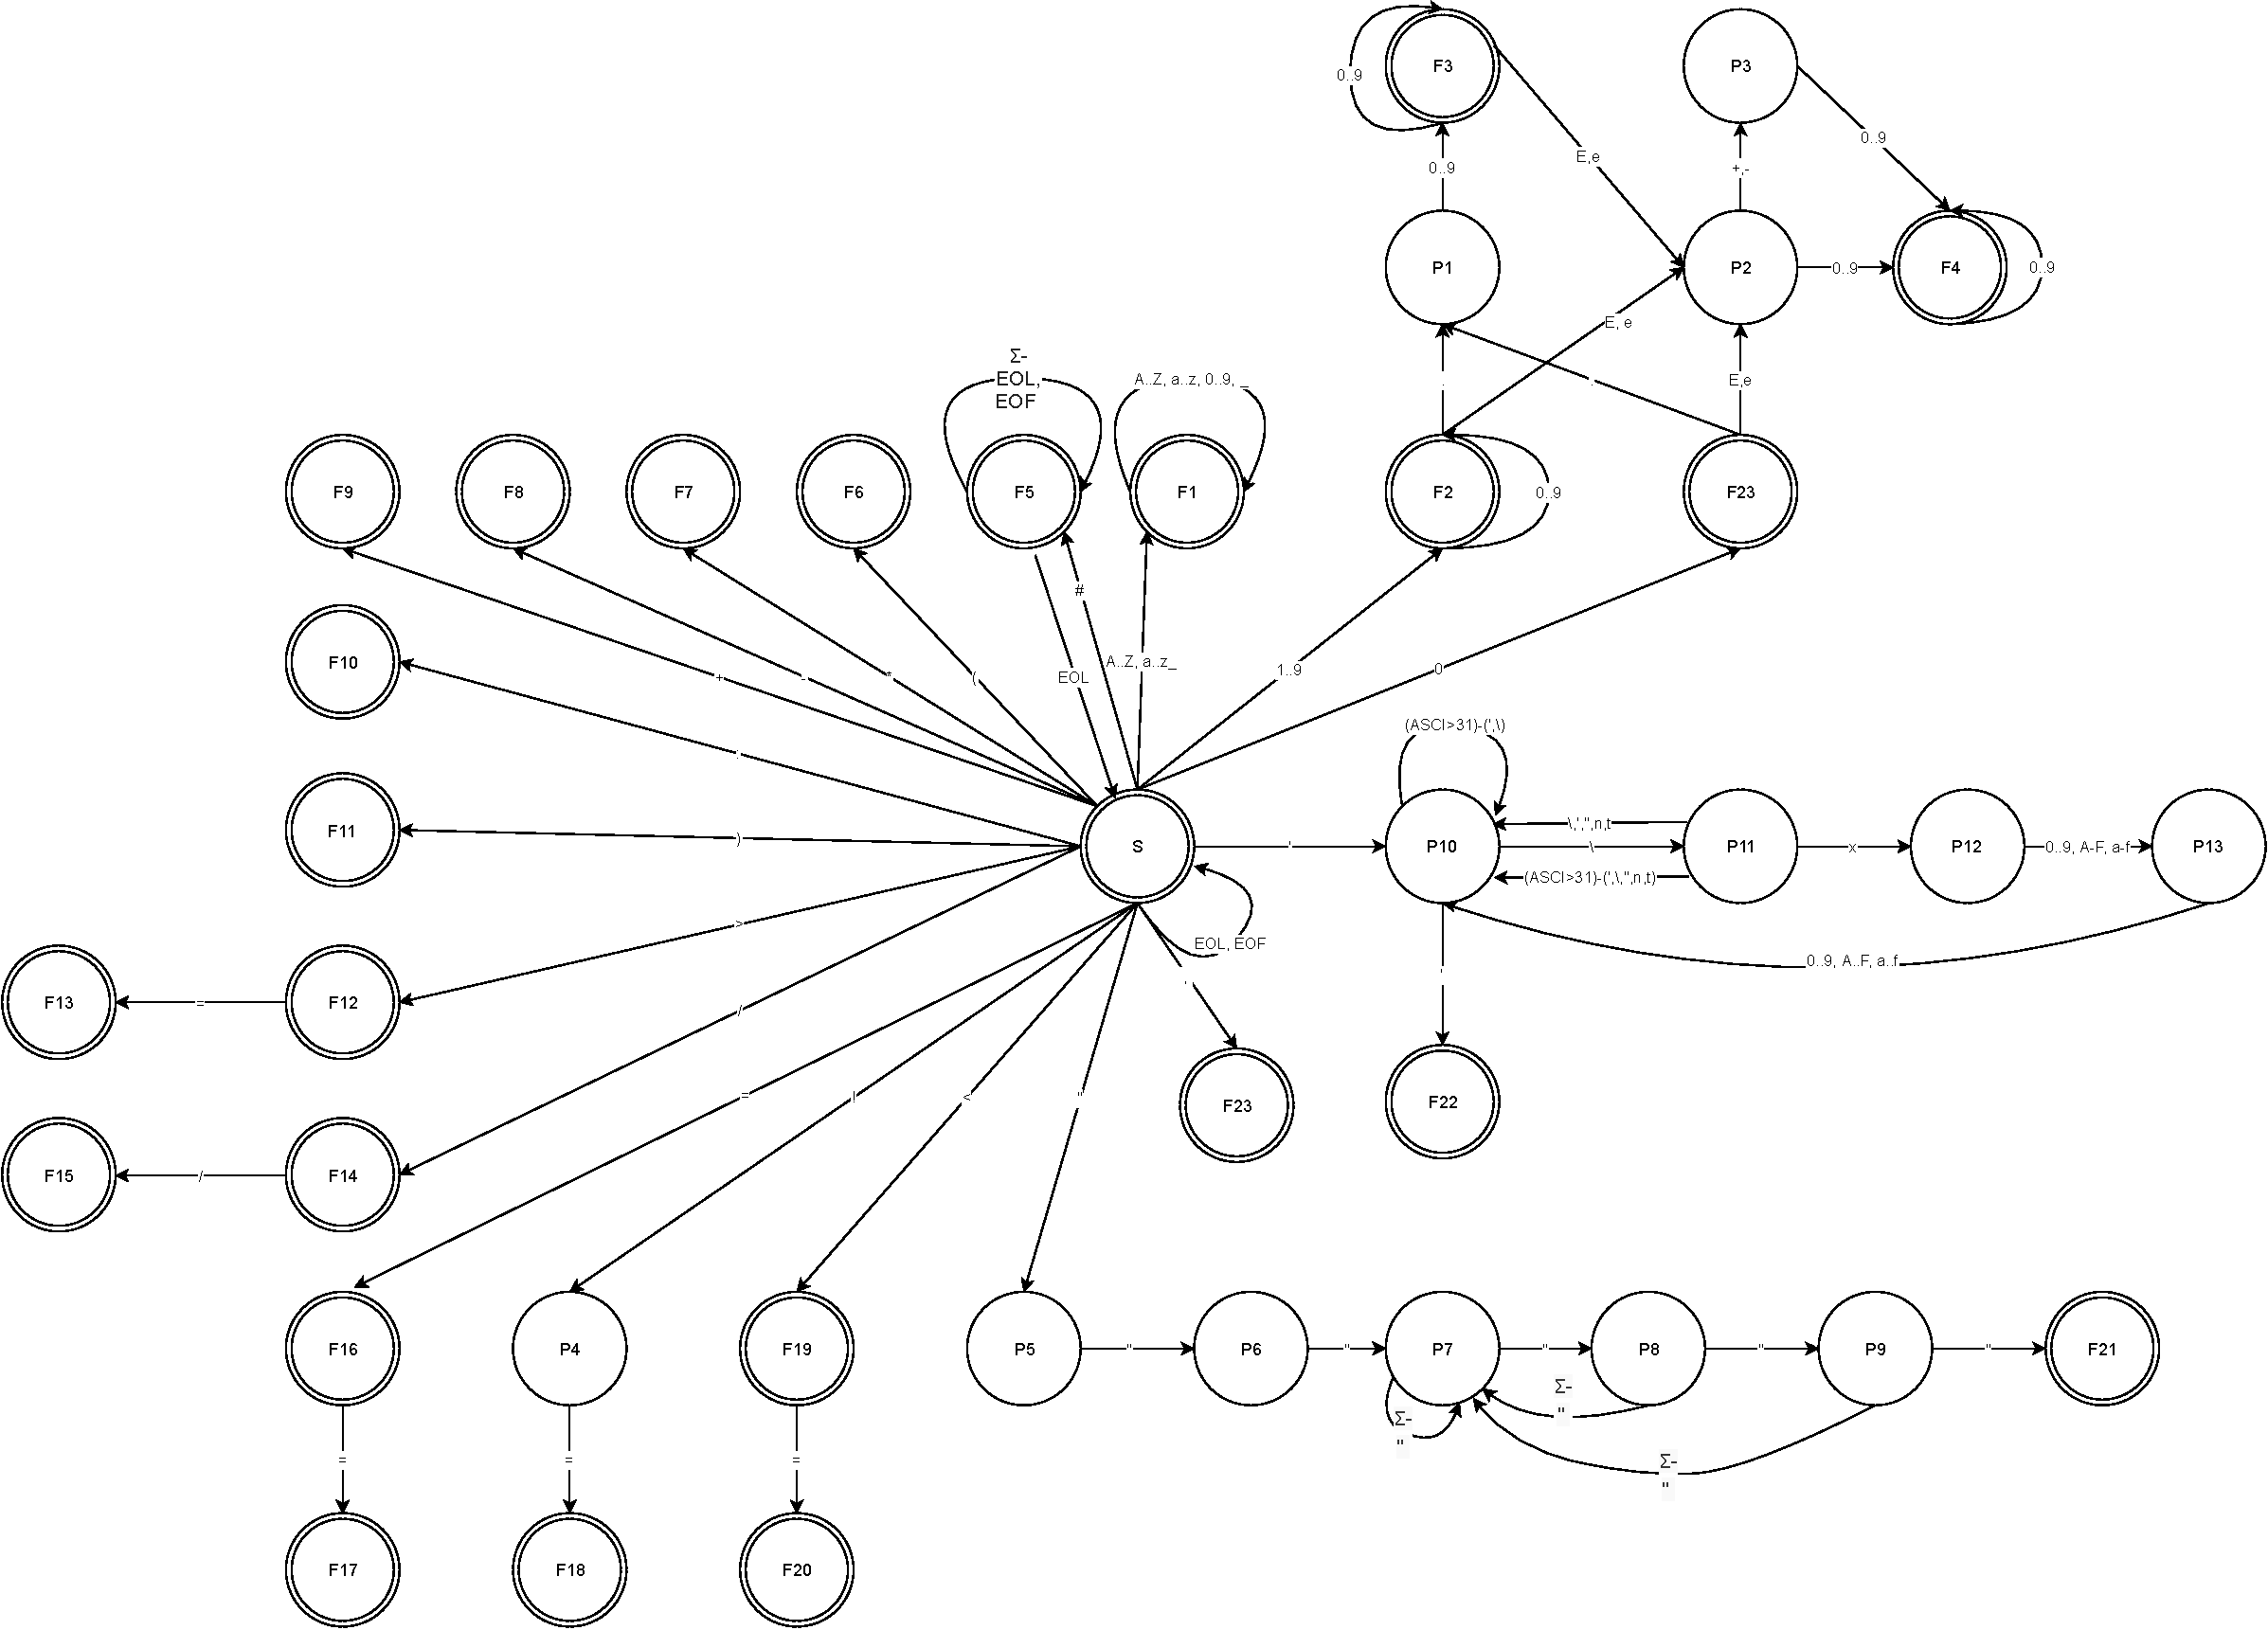
\includegraphics{src/FSM.pdf}} 
\caption{Diagram konečného automatu}\label{pic:1}
\end{figure}
\newpage

%%%%%%%%%%%%%%%%%%%%%%%%%% LEGENDA FSM %%%%%%%%%%%%%%%%%%%%%%%%%%%%%% 

\subsection{Legenda diagramu konečného automatu}
\begin{tabbing}
    \hspace*{2.75cm}\=\hspace*{1.25cm}\= \kill
    \textbf{Stav} \> \textbf{Popis}  \\
      P1    \>  integer point    \\
      P2    \>  exponent   \\
      P3    \>  exponent with sign  \\
      P4    \>  not equal  \\
      P5    \>  documentation string  \\
      P6    \>  documentation string  \\
      P7    \>  documentation string  \\
      P8    \>  documentation string  \\
      P9    \>  documentation string  \\
      P10   \>  string literal  \\
      P11   \>  string literal with (maybe) escape sequence  \\
      P12   \>  string literal with escape sequence with x  \\
      P13   \>  string literal with escape sequence with x and 1 hexadecimal number  \\
            \>    \\
      F1    \> identificator   \\
      F2    \> integer   \\
      F3    \> double   \\
      F4    \> number with exponent   \\
      F5    \> line comment   \\
      F6    \> left parentheses   \\
      F7    \> multiply   \\
      F8    \> minus   \\
      F9    \> plus   \\
      F10   \> colon   \\
      F11   \> right parentheses   \\
      F12   \> greater   \\
      F13   \> greater or equal   \\
      F14   \> divide float   \\
      F15   \> divide int   \\
      F16   \> equals   \\
      F17   \> compare   \\
      F18   \> completed not equal   \\
      F19   \> less   \\
      F20   \> less or equal   \\
      F21   \> completed documentation string   \\
      F22   \> completed string literal   \\
      F23   \> coma   \\
    
    \end{tabbing}


\newpage

%%%%%%%%%%%%%%%%%%%%%%%%%% PRECEDENC TABLE %%%%%%%%%%%%%%%%%%%%%%%%%%%%%% 

\section{Precedenční tabulka}
\begin{figure}[ht]
  \centering
    \scalebox{0.33}{\includegraphics{src/prec.png}} 
\caption{Precedenc table}\label{pic:2}
\end{figure}

%%%%%%%%%%%%%%%%%%%%%%%%%% LEGENDA PRECEDENCE TABLE %%%%%%%%%%%%%%%%%%%%%

\subsection{Legenda Precedenční tabulky}
\begin{itemize}
    \item r $=$ Relační operátory
    \item i $=$ Datové typy $($int, float, string$)$
\end{itemize}

\newpage

%%%%%%%%%%%%%%%%%%%%%%%%%% LL PRAVIDLA %%%%%%%%%%%%%%%%%%%%%%%%%%%%%% 

\section{LL gramatika}
    \verb|S| $\rightarrow$ \verb|DEFFUNC| \verb|S|   \\
    \verb|S| $\rightarrow$ \verb|STATEMENT| \verb|S| \\
    \verb|S| $\rightarrow$ eoftoken    \\
    \verb|DEFFUNC| $\rightarrow$  def str leftbracket \verb|DEFPARAMS| colon eol indent \verb|ENDOFDEFFUNC|   \\
    \verb|ENDOFDEFFUN|C $\rightarrow$ \verb|STATEMENT END|    \\
    \verb|ENDOFDEFFUNC| $\rightarrow$ return expression \verb|THIRDEND|   \\
    \verb|END| $\rightarrow$ dedent    \\
    \verb|END| $\rightarrow$ eoftoken  \\
    \verb|SECONDEND| $\rightarrow$ eol \\
    \verb|SECONDEND| $\rightarrow$eoftoken    \\
    \verb|THIRDEND| $\rightarrow$ eol dedent   \\
    \verb|THIRDEND| $\rightarrow$ eoftoken \\
    \verb|DEFPARAMS| $\rightarrow$ rightbracket    \\
    \verb|DEFPARAMS| $\rightarrow$ str \verb|DEFPARAMSN|  \\
    \verb|DEFPARAMSN| $\rightarrow$ rightbracket   \\
    \verb|DEFPARAMSN| $\rightarrow$ comma str \verb|DEFPARAMSN|   \\
    \verb|STATEMENT| $\rightarrow$ while expression colon eol indent \verb|STATEMENT STATEMENTS END|  \\
    \verb|STATEMENT| $\rightarrow$ if expression colon eol indent \verb|STATEMENT STATEMENTS| dedent else colon eol indent \verb|STATEMENT| $\rightarrow$ \verb|STATEMENTS END|   \\
    \verb|STATEMENT| $\rightarrow$ pass \verb|SECONDEND|  \\
    \verb|STATEMENT| $\rightarrow$ str \verb|STRINGTHINGIES|  \\
    \verb|STATEMENT| $\rightarrow$ expression  \\
    \verb|STATEMENT| $\rightarrow$ eol    \\
    \verb|STRINGTHINGIES| $\rightarrow$ leftbracket \verb|CALLPARAMS| \\
    \verb|STRINGTHINGIES| $\rightarrow$ assign expression \verb|SECONDEND|    \\
    \verb|CALLPARAMS| $\rightarrow$ rightbracket   \\
    \verb|CALLPARAMS| $\rightarrow$ str \verb|CALLPARAMSN|    \\
    \verb|CALLPARAMS| $\rightarrow$ float \verb|CALLPARAMSN|  \\
    \verb|CALLPARAMS| $\rightarrow$ int \verb|CALLPARAMSN|    \\
    \verb|CALLPARAMS| $\rightarrow$ doccom \verb|CALLPARAMSN| \\
    \verb|CALLPARAMS| $\rightarrow$ literal \verb|CALLPARAMSN|    \\
    \verb|CALLPARAMSN| $\rightarrow$ rightbracket  \\
    \verb|CALLPARAMSN| $\rightarrow$ comma \verb|AFTERCOMMA CALLPARAMSN|  \\
    \verb|AFTERCOMMA| $\rightarrow$ str    \\
    \verb|AFTERCOMMA| $\rightarrow$ float  \\
    \verb|AFTERCOMMA| $\rightarrow$ int    \\
    \verb|AFTERCOMMA| $\rightarrow$ literal    \\
    \verb|AFTERCOMMA| $\rightarrow$ doccom \\
 	\verb|STATEMENTS| $\rightarrow$ eps   \\
	\verb|STATEMENTS| $\rightarrow$ \verb|STATEMENT STATEMENTS|  \\
	\verb|S| $\rightarrow$ eps
	
	\begin{itemize}
        \item LL gramatika je využívaná při řízení syntaktické analýzy
    \end{itemize}
    
\newpage


%%%%%%%%%%%%%%%%%%%%%%%%%% LL TABLE %%%%%%%%%%%%%%%%%%%%%%%%%%%%%% 

\newpage
\begin{landscape}
\section{Tabulka LL gramatiky}
\begin{figure}[ht]
  \centering
   {\scalebox{0.63}{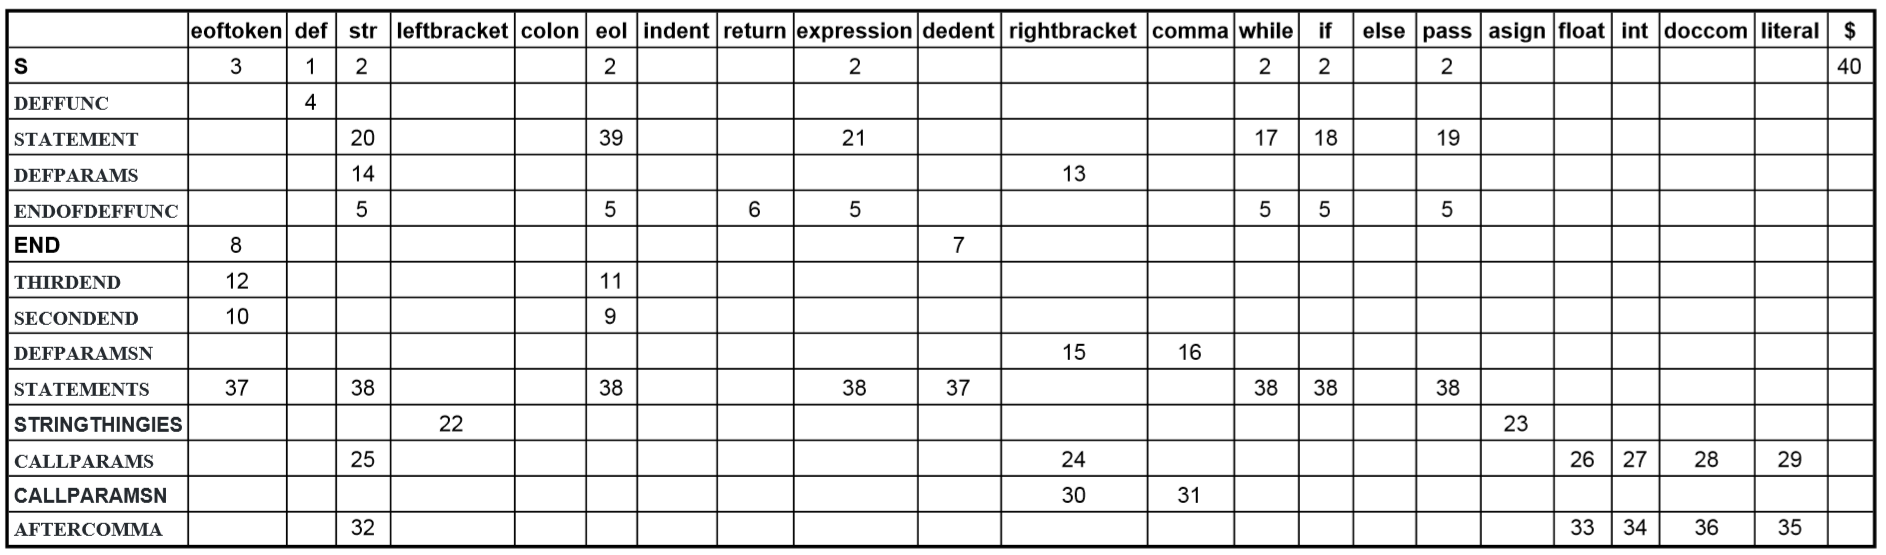
\includegraphics{src/LL.png}} }
\caption{Vygenerovaná tabulka LL gramatiky}\label{pic:3}
\end{figure}
\end{landscape}

\end{document}